\documentclass[aspectratio=169, 8pt]{beamer}
\usepackage[T2A]{fontenc}
\usepackage[utf8]{inputenc}
\usepackage[russian]{babel}
\usepackage{amsmath,amssymb,bm}
\usepackage{graphicx}
\usepackage{tikz}
\usepackage{booktabs}
\usepackage{array}
\usepackage{makecell}
\usetikzlibrary{arrows.meta, positioning, shapes, calc, fit, backgrounds, decorations.pathreplacing}

\usetheme{Ilmenau}
\usecolortheme{default}
\setbeamercolor{background canvas}{bg=white}
\setbeamercolor{normal text}{fg=black}
\setbeamercolor{frametitle}{fg=blue!80!black, bg=blue!5}
\setbeamercolor{title}{fg=white}
\setbeamercolor{item}{fg=blue!70}
\setbeamerfont{title}{size=\large, series=\bfseries}
\setbeamerfont{subtitle}{size=\normalsize}
\setbeamercolor{block title}{fg=white, bg=blue!60}
\setbeamercolor{block body}{bg=blue!5}
\setbeamercolor{alertblock title}{fg=white, bg=red!60}
\setbeamercolor{alertblock body}{bg=red!5}
\setbeamertemplate{navigation symbols}{}
\setbeamertemplate{footline}{
  \leavevmode
  \hbox{
    \begin{beamercolorbox}[wd=.5\paperwidth,ht=2ex,dp=1ex,left]{author in head/foot}
      \hspace*{1em}\insertshortauthor
    \end{beamercolorbox}
    \begin{beamercolorbox}[wd=.5\paperwidth,ht=2ex,dp=1ex,right]{date in head/foot}
      \insertframenumber{} / \inserttotalframenumber\hspace*{1em}
    \end{beamercolorbox}}
  \vskip0pt
}

\setlength{\abovedisplayskip}{3pt}
\setlength{\belowdisplayskip}{3pt}

\title{Языковые модели}
\subtitle{BERT, GPT, от RLHF до DeepSeek: как работают современные LLM}
\author{Курс «Deep Learning»}
\date{2026}

\begin{document}

% Slide 1
\begin{frame}
  \titlepage
\end{frame}

% Slide 2
\begin{frame}{Содержание}
  \begin{enumerate}
    \item Языковое моделирование: постановка задачи
    \item Encoder vs Decoder: два подхода
    \item Encoder-only: BERT
    \item Decoder-only: GPT
    \item Масштабирование: Scaling Laws
    \item Instruction Tuning и RLHF
    \item DeepSeek и Mixture of Experts
  \end{enumerate}
\end{frame}

% Slide 3
\begin{frame}{Языковое моделирование}
  \begin{columns}[T]
    \begin{column}{0.58\textwidth}
      \begin{block}{Задача}
        Предсказать вероятность последовательности токенов:
        \[
        P(w_1, w_2, \dots, w_n) = \prod_{t=1}^n P(w_t \mid w_{1:t-1})
        \]
      \end{block}
      \textbf{Цепное правило:} совместная вероятность = произведение условных.
      \textbf{Авторегрессия:} каждый следующий токен зависит от предыдущих.
      \vspace{0.2em}
      \begin{block}{Пример}
        $P(\text{«языковая»} \mid \text{«GPT — это»}) = 0.6$ \\
        $P(\text{«модель»} \mid \text{«GPT — это»}) = 0.3$ \\
        $P(\text{«очень»} \mid \text{«GPT — это»}) = 0.02$
      \end{block}
    \end{column}
    \begin{column}{0.42\textwidth}
      \begin{block}{Схема}
        \centering
        \begin{tikzpicture}[font=\footnotesize, node distance=0.5cm]
          \node[draw, fill=blue!10, thick, minimum width=0.8cm, minimum height=0.45cm] (t1) {GPT};
          \node[draw, fill=blue!10, thick, minimum width=0.8cm, minimum height=0.45cm, right=0.1cm of t1] (t2) {---};
          \node[draw, fill=blue!10, thick, minimum width=0.8cm, minimum height=0.45cm, right=0.1cm of t2] (t3) {это};
          \node[draw, fill=green!20, thick, minimum width=1.1cm, minimum height=0.45cm, right=0.1cm of t3] (t4) {$x_4$?};
          \draw[->, thick] (t1) -- (t2);
          \draw[->, thick] (t2) -- (t3);
          \draw[->, thick, dashed, red] (t3) -- (t4);
        \end{tikzpicture}
      \end{block}
      \begin{block}{Ключевые понятия}
        \textbf{Словарь $V$:} 32K--128K токенов (BPE/WordPiece) \\
        \textbf{Perplexity:} $2^{-\frac{1}{n}\sum \log_2 P(x_t)}$
      \end{block}
    \end{column}
  \end{columns}
\end{frame}

% Slide 4
\begin{frame}{Encoder vs Decoder: три парадигмы}
  \begin{columns}[T]
    \begin{column}{0.55\textwidth}
      \begin{block}{Encoder-only (BERT)}
        Маскированное языковое моделирование. Бидирекциональный контекст. \textbf{Понимание:} классификация, NER, QA.
        \vspace{0.3em}
        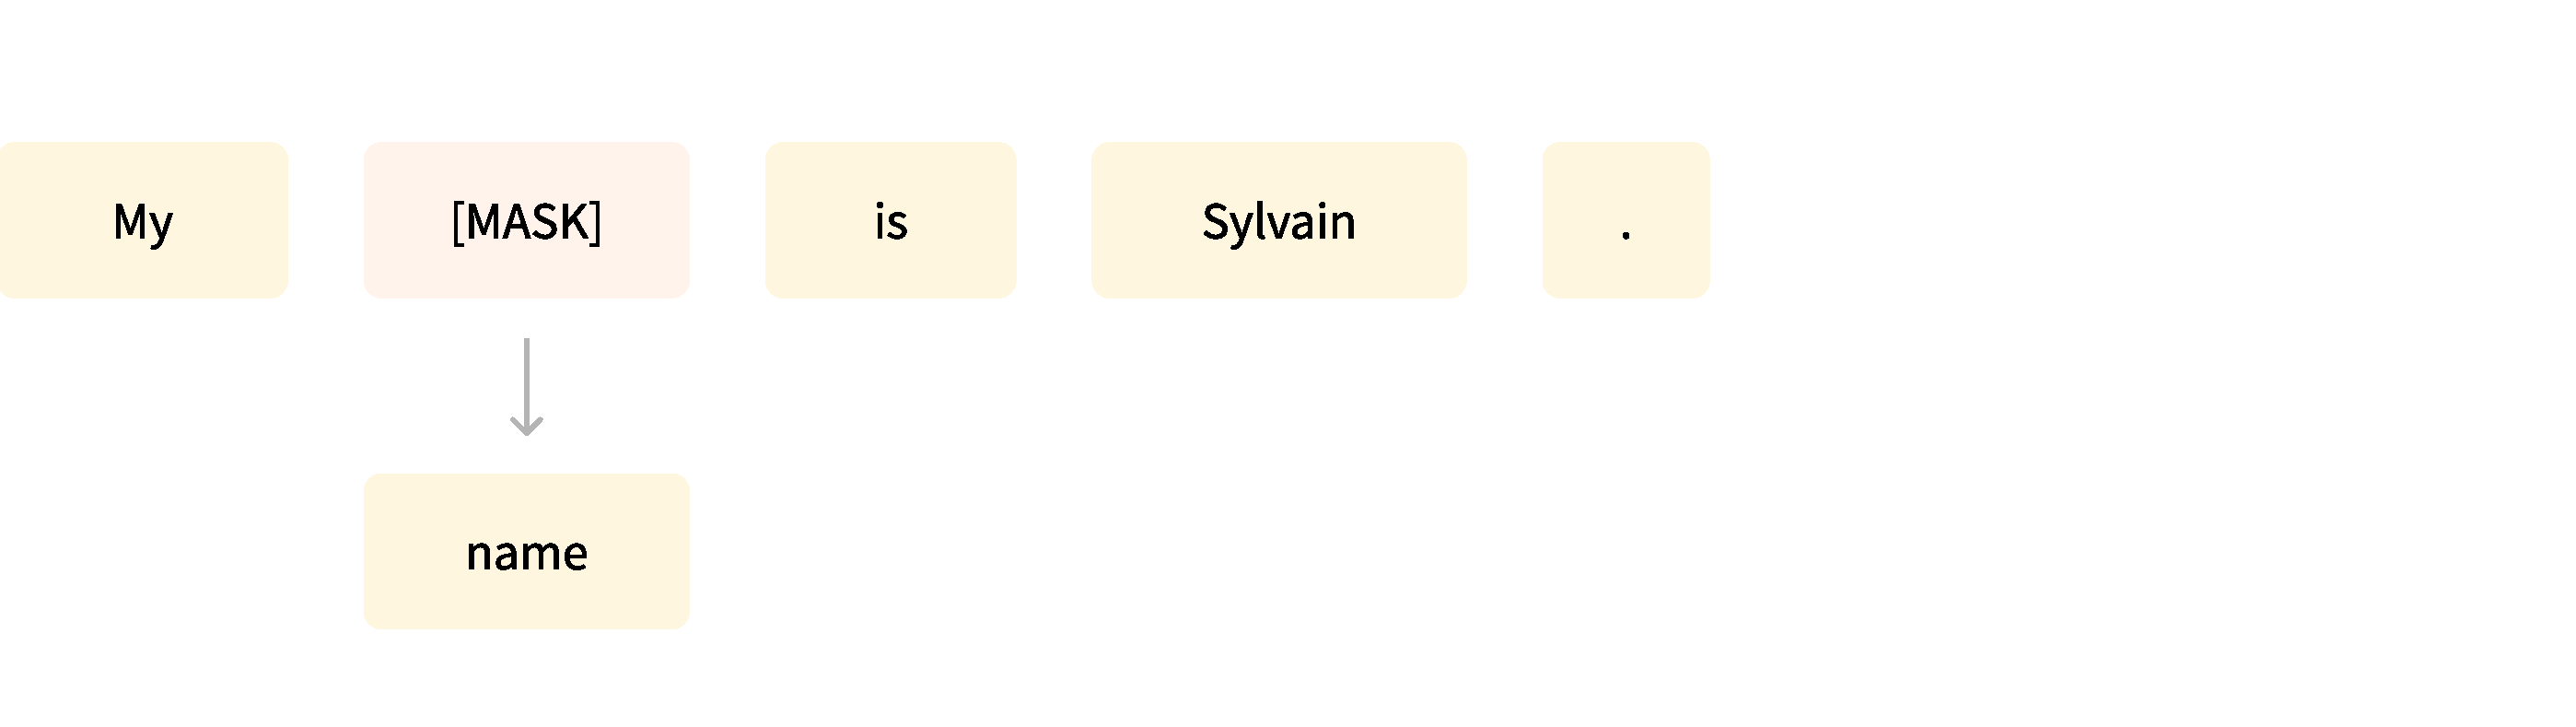
\includegraphics[width=\textwidth]{images/masked_modeling.pdf}
      \end{block}
    \end{column}
    \begin{column}{0.45\textwidth}
      \begin{block}{Decoder-only (GPT)}
        Авторегрессия (causal mask). \textbf{Генерация:} диалог, код, stories.
        \vspace{0.3em}
        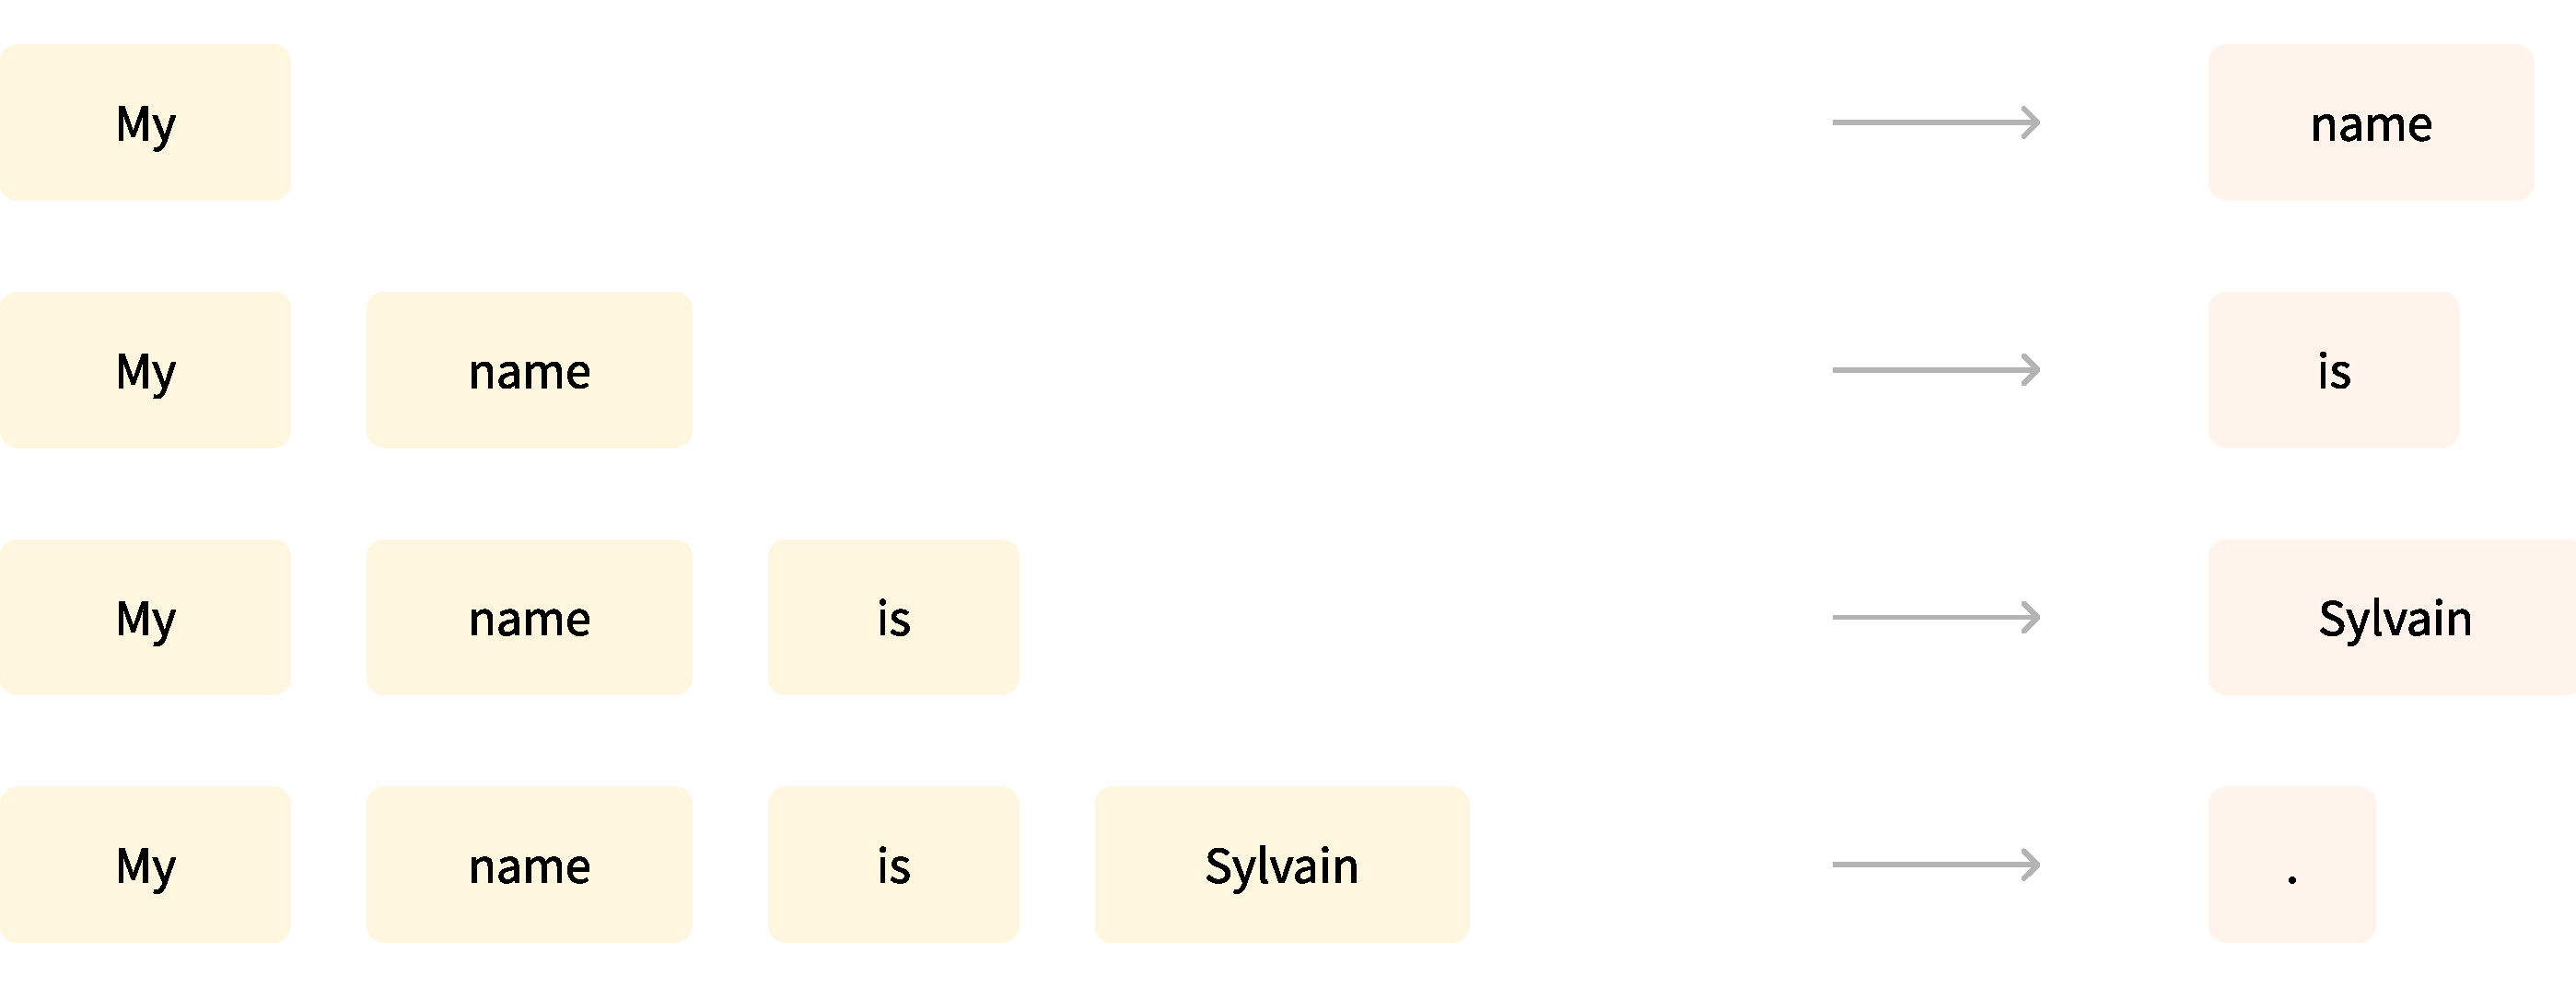
\includegraphics[width=\textwidth]{images/causal_modeling.pdf}
      \end{block}
    \end{column}
  \end{columns}
  \vspace{0.3em}
  \begin{block}{Encoder-Decoder (T5, BART)}
    Encoder читает вход (бидир.), Decoder генерирует (авторегр.). \textbf{Seq2Seq:} перевод, суммаризация.
  \end{block}
\end{frame}

% Slide 5
\begin{frame}{BERT: Encoder-only}
  \begin{columns}[T]
    \begin{column}{0.48\textwidth}
      \begin{block}{BERT = Bidirectional Encoder Representations from Transformers}
        \begin{itemize}
          \item Google, 2018 (Devlin et al.)
          \item Encoder-only, bi-directional контекст
        \end{itemize}
      \end{block}
      \textbf{Размеры:} Base: 110M (12 слоёв), Large: 340M (24 слоя)
      \begin{block}{Masked LM (MLM)}
        \texttt{The [MASK] sat on the mat $\to$ cat} \\
        15\% токенов маскируются: 80\% $\to$ [MASK], \\
        10\% $\to$ random, 10\% $\to$ original
      \end{block}
    \end{column}
    \begin{column}{0.52\textwidth}
      \begin{block}{Архитектура}
        \centering
        \begin{tikzpicture}[font=\footnotesize]
          \node[draw, fill=blue!20, minimum width=3.5cm, minimum height=0.5cm] at (0,1.7) {Transformer Encoder $\times N$};
          \node[draw, fill=blue!10, minimum width=0.8cm, minimum height=0.3cm] at (-1.5,0.3) {[CLS]};
          \node[draw, fill=blue!10, minimum width=0.8cm, minimum height=0.3cm] at (-0.5,0.3) {The};
          \node[draw, fill=red!20, minimum width=0.8cm, minimum height=0.3cm] at (0.5,0.3) {[MASK]};
          \node[draw, fill=blue!10, minimum width=0.8cm, minimum height=0.3cm] at (1.5,0.3) {mat};
          \foreach \x in {-1.5,-0.5,0.5,1.5}
            \draw[->] (\x,0.5) -- (\x,1.0);
          \node[draw, fill=green!20, minimum width=0.8cm, minimum height=0.3cm] at (0.5,2.6) {cat};
          \draw[->] (0.5,2.1) -- (0.5,2.35);
          \draw[<->, thick, blue] (-1.7,1.0) -- (1.7,1.0) node[midway, above, font=\tiny] {bi-directional};
        \end{tikzpicture}
      \end{block}
      \begin{block}{Next Sentence Prediction (NSP)}
        \texttt{[CLS] The cat sat [SEP] It was cute $\to$ IsNext}
      \end{block}
    \end{column}
  \end{columns}
\end{frame}

% Slide 6
\begin{frame}{BERT: Fine-tuning}
  \begin{columns}[T]
    \begin{column}{0.48\textwidth}
      \textbf{После предобучения} BERT донастраивается под конкретную задачу.
      \vspace{0.3em}
      \begin{block}{Классификация}
        [CLS]-токен $\to$ FC-слой $\to$ softmax. \\Тональность, спам, тематика.
      \end{block}
      \begin{block}{Token-level}
        Каждый выходной токен $\to$ FC-слой. \\NER, POS-теггинг, SQuAD (QA).
      \end{block}
    \end{column}
    \begin{column}{0.52\textwidth}
      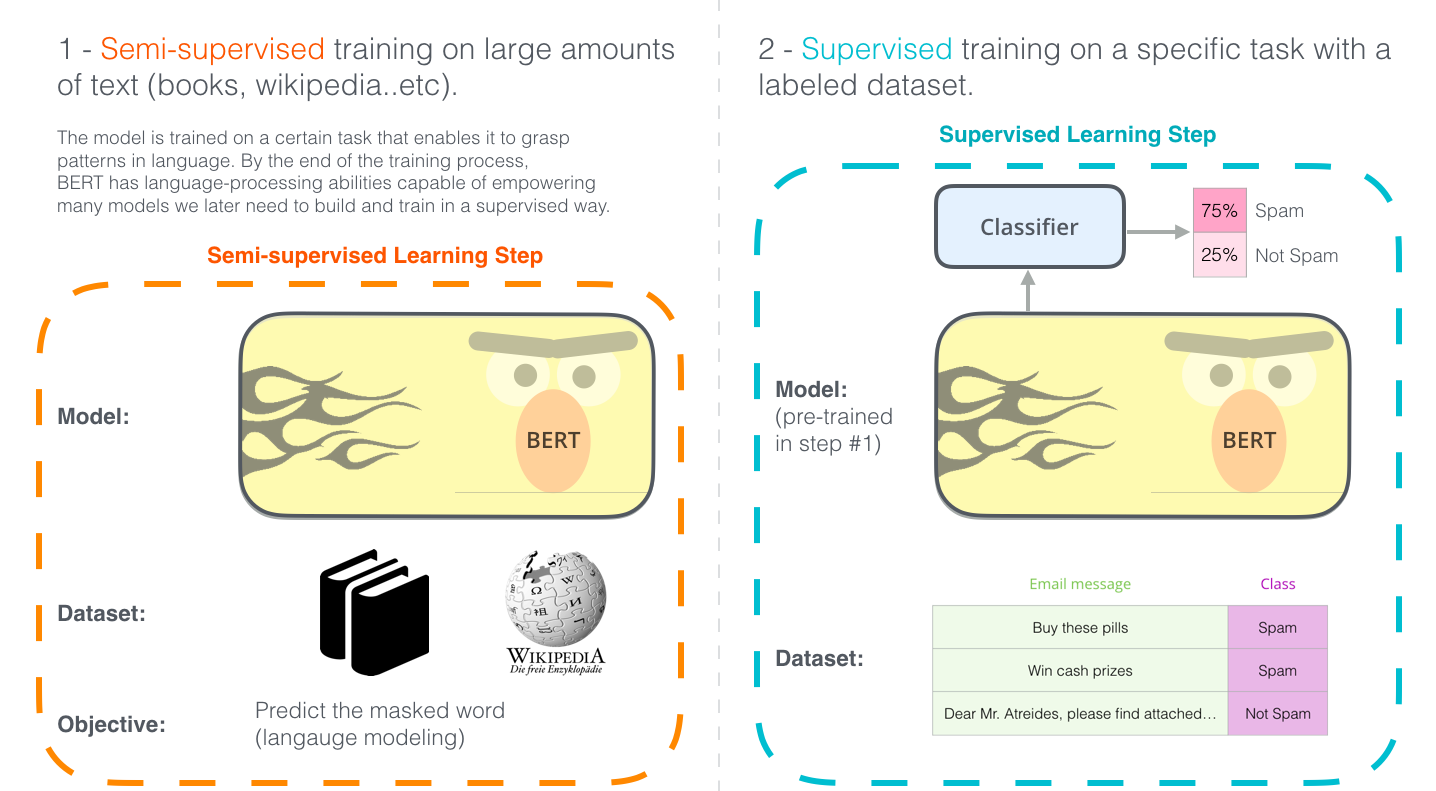
\includegraphics[width=\textwidth]{images/bert-transfer-learning.png}
      \vspace{0.2em}
      \centering\small Иллюстрация: Jay Alammar
    \end{column}
  \end{columns}
\end{frame}

% Slide 7
\begin{frame}{GPT: Decoder-only}
  \begin{columns}[T]
    \begin{column}{0.55\textwidth}
      \begin{block}{GPT = Generative Pre-trained Transformer}
        \begin{itemize}
          \item OpenAI, 2018 (Radford et al.)
          \item Decoder-only, causal mask
          \item Токен видит только предыдущие
          \item Предобучение: next token prediction
        \end{itemize}
      \end{block}
      \textbf{Эволюция:}
      \begin{tabular}{lrl}
        \toprule
        \textbf{Модель} & \textbf{Параметры} & \textbf{Слои} \\
        \midrule
        GPT-1 (2018) & 117M & 12 \\
        GPT-2 (2019) & 1.5B & 48 \\
        GPT-3 (2020) & 175B & 96 \\
        GPT-4 (2023) & $\approx$1.7T & ? (MoE) \\
        \bottomrule
      \end{tabular}
      \vspace{0.2em}
      \begin{alertblock}{Ключевое отличие}
        BERT --- bi-directional. GPT --- uni-directional (causal).
      \end{alertblock}
    \end{column}
    \begin{column}{0.45\textwidth}
      \begin{block}{Архитектура GPT (decoder-only)}
        \centering
        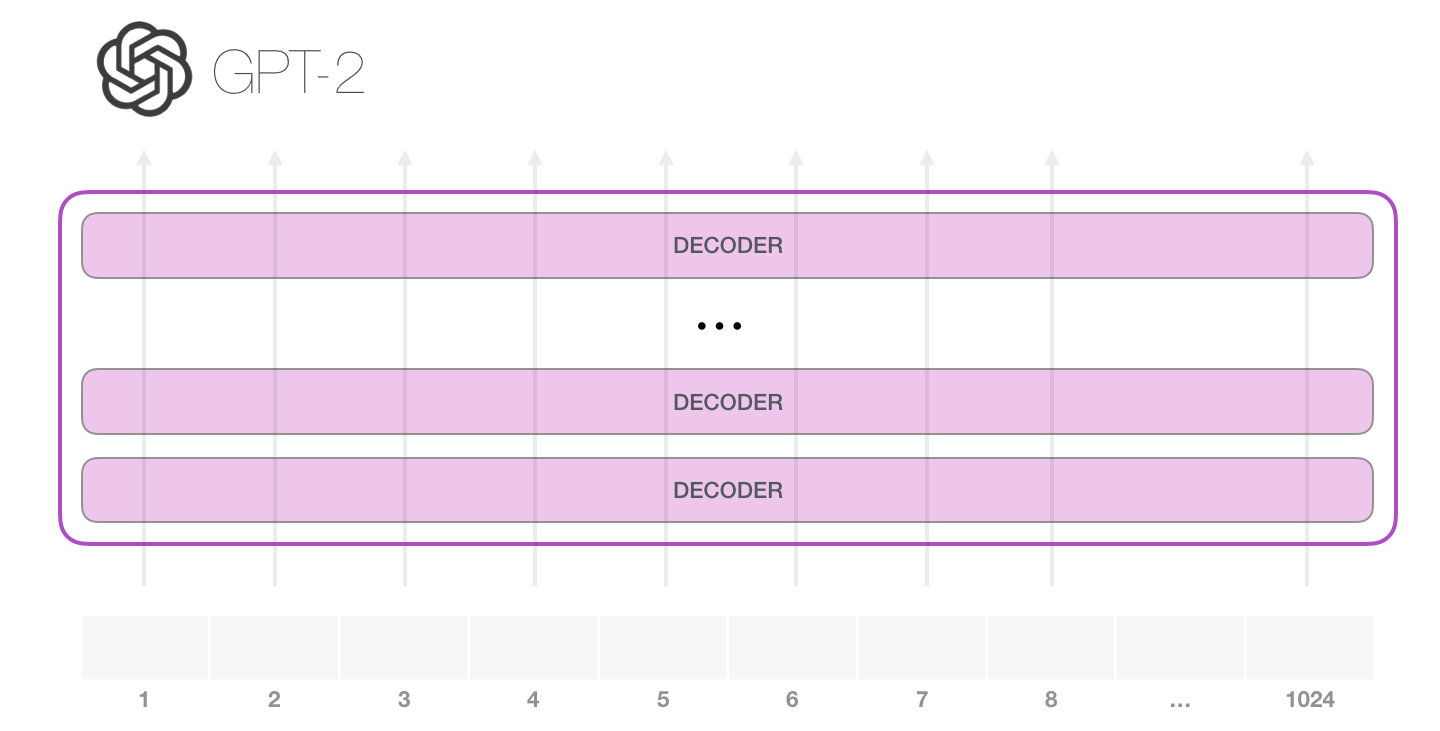
\includegraphics[width=\textwidth]{images/gpt-2-layers-2.png}
        \vspace{0.1em}\\
        {\tiny Иллюстрация: Jay Alammar, The Illustrated GPT-2}
      \end{block}
      \vspace{0.1em}
      \textbf{Функция потерь:}
      \[
      \mathcal{L} = -\frac{1}{T}\sum_{t=1}^T \log P(x_t \mid x_{<t}; \theta)
      \]
    \end{column}
  \end{columns}
\end{frame}

% Slide 8
\begin{frame}{Обучение GPT: данные и оптимизация}
  \begin{columns}[T]
    \begin{column}{0.48\textwidth}
      \begin{block}{Подготовка данных}
        \begin{itemize}
          \item Common Crawl, WebText, Wikipedia, книги
          \item Токенизация BPE (Byte Pair Encoding)
          \item Конкатенация с [EOS]-токенами
          \item Варианты: Pile, C4, RefinedWeb
        \end{itemize}
      \end{block}
      \begin{block}{Один шаг}
        \texttt{GPT is a ??? $\to$ target: \textcolor{red}{transformer}}
      \end{block}
    \end{column}
    \begin{column}{0.52\textwidth}
      \begin{block}{Параметры обучения}
        \begin{tabular}{ll}
          \toprule
          \textbf{Параметр} & \textbf{Значение} \\
          \midrule
          Оптимизатор & AdamW ($\beta_1=0.9$, $\beta_2=0.95$) \\
          LR schedule & Cosine decay + warmup \\
          Max LR & $3\times 10^{-4}$ (GPT-3 175B) \\
          Batch size & 3.2M токенов \\
          Weight decay & 0.1 \\
          Gradient clipping & 1.0 \\
          Precision & FP16 / BF16 / FP8 \\
          \bottomrule
        \end{tabular}
      \end{block}
      \begin{alertblock}{Chinchilla}
        GPT-3 (175B) обучался на 300B токенов. Нужно $\approx 20\times$ больше токенов, чем параметров.
      \end{alertblock}
    \end{column}
  \end{columns}
\end{frame}

% Slide 9
\begin{frame}{Инференс GPT}
  \begin{columns}[T]
    \begin{column}{0.48\textwidth}
      \begin{block}{Авторегрессия}
        Prompt $\to$ GPT $\to$ [logits] $\to$ [sampling] $\to$ next token. Добавить, повторить.
      \end{block}
      \begin{block}{KV Cache}
        \begin{itemize}
          \item Сохраняем $K$ и $V$ на каждом слое
          \item На новом шаге: только новый токен
          \item $O(n^2) \to O(n)$ на токен
        \end{itemize}
      \end{block}
    \end{column}
    \begin{column}{0.52\textwidth}
      \begin{block}{Стратегии декодирования}
        \begin{tabular}{lll}
          \toprule
          \textbf{Метод} & \textbf{Описание} & \textbf{Хар-ка} \\
          \midrule
          Greedy & $\arg\max P$ & просто, циклы \\
          Top-$k$ & ресемплинг из $k$ & $k=40$--100 \\
          Top-$p$ & nucleus: кум. $p$ & $p=0.9$--0.95 \\
          Temperature & $P\propto e^{l/T}$ & $T=0.7$--1.0 \\
          Beam search & $k$ гипотез & перевод \\
          \bottomrule
        \end{tabular}
      \end{block}
    \end{column}
  \end{columns}
\end{frame}

% Slide 10
\begin{frame}{От GPT-1 к GPT-4: масштабирование}
  \centering
  \begin{tikzpicture}[font=\small]
    \draw[->] (0,0) -- (11.5,0) node[right] {Размер модели $\to$};
    \draw[->] (0,0) -- (0,3.2) node[above] {Способности $\to$};

    \node[fill=red!20, draw, minimum width=1.8cm, minimum height=0.5cm] (g1) at (1.2,1.0) {GPT-1};
    \node[fill=red!30, draw, minimum width=1.8cm, minimum height=0.5cm] (g2) at (3.5,1.5) {GPT-2};
    \node[fill=red!50, draw, minimum width=1.8cm, minimum height=0.5cm] (g3) at (6.5,2.0) {GPT-3};
    \node[fill=red!70, draw, minimum width=1.8cm, minimum height=0.5cm] (g4) at (9.5,2.6) {GPT-4};

    \node[font=\tiny, below=0.35cm of g1] {117M};
    \node[font=\tiny, below=0.35cm of g2] {1.5B};
    \node[font=\tiny, below=0.35cm of g3] {175B};
    \node[font=\tiny, below=0.35cm of g4] {$\approx$1.7T};

    \draw[red, thick, domain=0:10.7] plot (\x, {0.2 + 0.22*\x});
    \fill[green!80!black] (5.5,1.9) circle (3pt) node[above, font=\tiny, text=green!80!black] {Emergent abilities};
    \draw[dashed] (5,0) -- (5,2.8);
    \node[font=\tiny, below, text=green!80!black] at (5,0) {Порог emergent};
  \end{tikzpicture}

  \vspace{0.2em}
  \begin{columns}[T]
    \begin{column}{0.33\textwidth}
      \begin{block}{In-Context Learning}
        Few-shot примеры в промпте. GPT-2 не мог, GPT-3 --- да.
      \end{block}
    \end{column}
    \begin{column}{0.34\textwidth}
      \begin{block}{Chain-of-Thought}
        «Давайте подумаем шаг за шагом» $\to$ рассуждения.
      \end{block}
    \end{column}
    \begin{column}{0.33\textwidth}
      \begin{block}{Few-shot}
        Zero / one / few-shot. Точность растёт с числом примеров.
      \end{block}
    \end{column}
  \end{columns}
\end{frame}

% Slide 11
\begin{frame}{Scaling Laws}
  \begin{columns}[T]
    \begin{column}{0.48\textwidth}
      \begin{block}{Kaplan et al., 2020}
        $\text{Loss} \propto N^{-0.076} \cdot D^{-0.103}$
        \begin{itemize}
          \item Степенной закон от $N$ и $D$
          \item $N$ важнее $D$ (при фикс. бюджете)
        \end{itemize}
      \end{block}
      \begin{block}{Chinchilla (Hoffmann et al., 2022)}
        \begin{itemize}
          \item Для 175B нужно $\approx 3.7$T токенов
          \item Chinchilla 70B / 1.4T $>$ GPT-3 175B
        \end{itemize}
      \end{block}
    \end{column}
    \begin{column}{0.52\textwidth}
      \begin{block}{Параметры : Токены}
        \begin{tabular}{lcc}
          \toprule
          \textbf{Модель} & \textbf{Параметры} & \textbf{Токены} \\
          \midrule
          GPT-3 & 175B & 300B ($1.7\times$) \\
          Chinchilla & 70B & 1.4T ($20\times$) \\
          LLaMA 65B & 65B & 1.4T ($21.5\times$) \\
          DeepSeek-V3 & 671B & 14.8T ($22\times$) \\
          \bottomrule
        \end{tabular}
      \end{block}
      \vspace{0.2em}
      \begin{alertblock}{Вывод}
        Большинство моделей недообучены. Стандарт: $\approx 20\times$ больше токенов, чем параметров.
      \end{alertblock}
    \end{column}
  \end{columns}
\end{frame}

% Slide 12
\begin{frame}{Instruction Tuning}
  \begin{columns}[T]
    \begin{column}{0.48\textwidth}
      \begin{block}{Проблема}
        Raw GPT-3 продолжает текст, а не следует инструкциям. \\
        \texttt{Переведи: Hello $\to$ «Hello» может быть...} \\
        А нужно: \texttt{Здравствуйте}
      \end{block}
      \textbf{Решение:} SFT на парах (инструкция, ответ).
      \begin{block}{SFT workflow}
        \begin{tikzpicture}[font=\footnotesize]
          \node[draw, fill=blue!10, minimum width=3.5cm, minimum height=0.4cm] (raw) {Raw GPT};
          \draw[->] (raw) -- ++(0,0.35);
          \node[draw, fill=orange!20, minimum width=3.5cm, minimum height=0.4cm] (sft) {SFT};
          \draw[->] (sft) -- ++(0,0.35);
          \node[draw, fill=green!20, minimum width=3.5cm, minimum height=0.4cm] (fin) {Instruction-tuned};
        \end{tikzpicture}
      \end{block}
    \end{column}
    \begin{column}{0.52\textwidth}
      \begin{block}{Датасеты}
        \begin{itemize}
          \item \textbf{FLAN:} 60+ NLP-задач $\to$ инструкции
          \item \textbf{Alpaca:} 52K инструкций от GPT-3.5
          \item \textbf{OpenAssistant:} краудсорсинг
        \end{itemize}
      \end{block}
      \begin{block}{Формат диалога}
        \texttt{<|system|> Ты полезный ассистент} \\
        \texttt{<|user|> Переведи: Hello} \\
        \texttt{<|assistant|> Здравствуйте}
      \end{block}
      \textbf{Ограничение:} SFT решает follow instructions, но не alignment.
    \end{column}
  \end{columns}
\end{frame}

% Slide 13
\begin{frame}{RLHF: трёхшаговый pipeline}
  \centering
  \begin{tikzpicture}[font=\small]
    \node[draw, fill=blue!20, minimum width=2.8cm, minimum height=0.6cm] (sft) at (0,1.5) {\textbf{1. SFT}};
    \node[draw, fill=orange!20, minimum width=2.8cm, minimum height=0.6cm] (rm) at (4,1.5) {\textbf{2. Reward Model}};
    \node[draw, fill=green!20, minimum width=2.8cm, minimum height=0.6cm] (ppo) at (8,1.5) {\textbf{3. PPO}};
    \draw[->, thick] (1.5,1.5) -- (2.5,1.5);
    \draw[->, thick] (5.5,1.5) -- (6.5,1.5);
    \node[font=\tiny, below=0.1cm of sft] {Fine-tune на инструкциях};
    \node[font=\tiny, below=0.1cm of rm] {Обучаем оценщик};
    \node[font=\tiny, below=0.1cm of ppo] {RL с наградой от RM};
  \end{tikzpicture}

  \vspace{0.1em}
  \begin{columns}[T]
    \begin{column}{0.33\textwidth}
      \textbf{1. SFT} \\
      \small
      \begin{itemize}
        \item Пара (промпт, ответ)
        \item Next-token loss
        \item 10K--100K примеров
      \end{itemize}
    \end{column}
    \begin{column}{0.34\textwidth}
      \textbf{2. Reward Model} \\
      \small
      \begin{itemize}
        \item Несколько ответов \\
        $\to$ Человек: A$>$B$>$C
        \item $P(A>B)=\sigma(r_A-r_B)$
      \end{itemize}
    \end{column}
    \begin{column}{0.33\textwidth}
      \textbf{3. PPO} \\
      \small
      \begin{itemize}
        \item RL с наградой от RM
        \item KL penalty к SFT
        \item $\mathcal{L}= \mathbb{E}[-r] + \beta D_{KL}$
      \end{itemize}
    \end{column}
  \end{columns}

  \vspace{0.2em}
  \textbf{Пример обучения RM:} \\
  \texttt{Prompt $\to$ [Ответ A] [Ответ B] [Ответ C]} \\
  \texttt{Человек: B $>$ A $>$ C $\to$ RM учится}
\end{frame}

% Slide 14
\begin{frame}{От InstructGPT к ChatGPT}
  \begin{columns}[T]
    \begin{column}{0.45\textwidth}
      \begin{block}{InstructGPT (Ouyang et al., 2022)}
        \begin{itemize}\small
          \item GPT-3 $\to$ SFT на 13K инструкций
          \item RM на 33K сравнений
          \item PPO fine-tuning
          \item \textbf{Результат:} 1.3B $>$ 175B GPT-3
        \end{itemize}
      \end{block}
      \textbf{Ключевой инсайт:} alignment $>$ размер модели.
    \end{column}
    \begin{column}{0.55\textwidth}
      \begin{block}{ChatGPT (Nov 2022)}
        \begin{itemize}\small
          \item SFT + RM + PPO на диалогах
          \item Multi-turn, safety
          \item Роли: system/user/assistant
        \end{itemize}
      \end{block}
      \begin{block}{Альтернативы RLHF}
        \begin{tabular}{ll}
          \textbf{DPO (2023)} & Прямая оптимизация без RM и RL \\
          \textbf{GRPO} & Без Critic-сети (DeepSeek) \\
          \textbf{Constitutional AI} & Самооценка по правилам \\
          \textbf{RLAIF} & RM $\to$ LLM-фидбек \\
        \end{tabular}
      \end{block}
    \end{column}
  \end{columns}
\end{frame}

% Slide 15
\begin{frame}{DeepSeek: Reasoning через RL}
  \begin{columns}[T]
    \begin{column}{0.48\textwidth}
      \begin{block}{DeepSeek-R1 (январь 2025)}
        \textbf{Идея:} обучение рассуждению через RL, без SFT.
        \begin{enumerate}\small
          \item Cold-start: небольшой SFT
          \item GRPO: награда за ответ + формат
          \item Self-evolution: CoT emerges
        \end{enumerate}
      \end{block}
      \textbf{GRPO:} без Critic-сети. Оценка по группе ответов.
    \end{column}
    \begin{column}{0.52\textwidth}
      \begin{block}{DeepSeek-V3 (декабрь 2024)}
        \begin{itemize}\small
          \item 671B пар., 37B активных (MoE, 256 экспертов)
          \item 14.8T токенов, FP8
          \item Multi-Token Prediction
          \item \textbf{Стоимость:} \$5.5M ($10\times$ дешевле)
        \end{itemize}
      \end{block}
      \begin{block}{Архитектурные решения}
        \begin{itemize}\small
          \item MLA: сжатие KV кеша в $4\times$
          \item Мелкозернистые эксперты
          \item Shared expert + loss-free balancing
        \end{itemize}
      \end{block}
    \end{column}
  \end{columns}
\end{frame}

% Slide 16
\begin{frame}{Mixture of Experts (MoE)}
  \begin{columns}[T]
    \begin{column}{0.55\textwidth}
      \begin{block}{Dense vs MoE}
        \begin{tikzpicture}[font=\small]
          \node[draw, fill=blue!20, minimum width=2.8cm, minimum height=0.5cm] (d1) at (-2.5,0.8) {FFN};
          \draw[->] (-2.5,1.3) -- (d1);
          \draw[->] (d1) -- (-2.5,0.3);
          \node[below, font=\tiny] at (-2.5,-0.1) {Dense: 1 FFN};

          \node[draw, fill=orange!20, minimum width=1.2cm, minimum height=0.35cm] (gate) at (1.8,1.1) {Gating};
          \foreach \x/\l in {0.3/E1,1.0/E2,1.8/E3,2.6/E4,3.3/E5} {
            \node[draw, fill=green!10, minimum width=0.6cm, minimum height=0.3cm, font=\tiny] at (\x,0.5) {\l};
          }
          \node[below, font=\tiny] at (1.8,-0.1) {MoE: top-2 активны};
          \draw[->] (gate.south) -- (1.0,0.65);
          \draw[->] (gate.south) -- (2.6,0.65);
          \draw[->] (1.8,1.5) -- (gate);
        \end{tikzpicture}
      \end{block}
      \textbf{Формула:} MoE$(x) = \sum_i G(x)_i \cdot E_i(x)$, $G(x) = \text{softmax}(W_g x)$
    \end{column}
    \begin{column}{0.45\textwidth}
      \begin{block}{Плюсы / Минусы}
        \textbf{+} Больше параметров, те же FLOPs \\
        \textbf{+} Качество $\approx$ dense полного размера \\
        \textbf{--} Все эксперты в VRAM \\
        \textbf{--} Load balancing, сложный fine-tuning
      \end{block}
      \begin{block}{Примеры}
        \begin{tabular}{lrr}
          \toprule
          \textbf{Модель} & \textbf{Всего} & \textbf{Активно} \\
          \midrule
          Mixtral 8x7B & 47B & 12.9B \\
          DeepSeek-V2 & 236B & 21B \\
          DeepSeek-V3 & 671B & 37B \\
          GPT-4 (rum.) & $\approx$1.7T & $\approx$200B \\
          \bottomrule
        \end{tabular}
      \end{block}
    \end{column}
  \end{columns}
\end{frame}

% Slide 17
\begin{frame}{Современные тренды LLM}
  \begin{columns}[T]
    \begin{column}{0.33\textwidth}
      \begin{block}{Architecture}
        \begin{itemize}\small
          \item MoE --- новый стандарт
          \item MQA / GQA attention
          \item RoPE, ALiBi embeddings
          \item Mamba / SSM
        \end{itemize}
      \end{block}
      \begin{block}{Inference}
        \begin{itemize}\small
          \item KV cache quantization
          \item Speculative decoding
          \item Continuous batching
        \end{itemize}
      \end{block}
    \end{column}
    \begin{column}{0.33\textwidth}
      \begin{block}{Training}
        \begin{itemize}\small
          \item FP8 / mixed precision
          \item Multi-Token Prediction
          \item Curriculum learning
          \item Data quality $>$ quantity
        \end{itemize}
      \end{block}
      \begin{block}{Reasoning}
        \begin{itemize}\small
          \item Chain-of-Thought
          \item Test-time compute scaling
          \item Agentic AI / tool use
        \end{itemize}
      \end{block}
    \end{column}
    \begin{column}{0.33\textwidth}
      \begin{block}{Alignment}
        \begin{itemize}\small
          \item DPO, GRPO
          \item Constitutional AI
          \item RLAIF
          \item Safety at scale
        \end{itemize}
      \end{block}
      \begin{block}{Open Source}
        \begin{itemize}\small
          \item LLaMA, Qwen, DeepSeek
          \item Mixtral, Command R+
        \end{itemize}
      \end{block}
    \end{column}
  \end{columns}
\end{frame}

% Slide 18
\begin{frame}{Заключение}
  \begin{columns}[T]
    \begin{column}{0.5\textwidth}
      \textbf{Что мы узнали:}
      \begin{itemize}\small
        \item LM: $P(\text{next} \mid \text{context})$
        \item BERT: encoder, bi-directional, MLM
        \item GPT: decoder, авторегрессия, KV cache
        \item Scaling Laws: $N + D =$ качество
        \item RLHF: SFT $\to$ RM $\to$ PPO
        \item DeepSeek: reasoning + MoE
      \end{itemize}
    \end{column}
    \begin{column}{0.5\textwidth}
      \begin{block}{Ключевые идеи}
        \begin{itemize}\small
          \item \textbf{Emergent:} способности при масштабировании
          \item \textbf{Alignment:} маленькая aligned $>$ большая
          \item \textbf{Sparsity:} MoE --- больше за те же FLOPs
        \end{itemize}
      \end{block}
      \textbf{Дальше:} мультимодальные модели, агенты, video gen.
    \end{column}
  \end{columns}
\end{frame}

\end{document}
